\documentclass{article}
\usepackage[utf8]{inputenc}

\title{Baza de date a Uniunii Asociațiilor Europene de Fotbal (UEFA) Sezonul 2015/2016}
\author{Vaidacuțean Georgiana Denisa Nicoleta \\ Seria 13, grupa 131}
\date{\today}
\usepackage{indentfirst}
\usepackage{enumitem}
\usepackage[a4paper, margin=2cm]{geometry}
\usepackage{setspace}
\usepackage{graphicx}

\onehalfspacing

\begin{document}
	\sloppy
	\maketitle
	
	\newpage
	
	\section{Introducere}
	\subsection{Descrierea modelului real și a utilității acestuia}
	
	Modelul de bază de date aferent Uniunii Asociațiilor Europene de Fotbal (UEFA) este conceput pentru a susține gestionarea informațiilor referitoare atât la campionatele interne organizate la nivelul statelor membre, cât și la competițiile internaționale de fotbal desfășurate în spațiul european, aflate sub coordonarea și reglementarea UEFA.
	
	Prin acest model, se urmărește organizarea eficientă a datelor despre echipe, jucători, meciuri și scoruri, având în vedere atât competițiile de club, cât și Campionatul European de Fotbal disputat între echipele naționale masculine de seniori ale membrilor UEFA.
	
	\vspace{0.5cm}
	
	\textit{Modelul este raportat la sezonul competițional 2015-2016, care include UEFA Champions League, UEFA Europa League și turneul final al Campionatului European desfășurat în vara anului 2016.}
	
	\vspace{0.3cm}
	
	\subsection{Principii generale de desfășurare}
	
	Fiecare țară membră UEFA găzduiește propriul campionat intern de fotbal, iar gestionarea acestuia este responsabilitatea asociației naționale de fotbal a respectivei țări. Asociația stabilește regulile și structura competiției, inclusiv numărul de echipe participante, formatul de desfășurare și calendarul meciurilor, asigurându-se că toate echipele respectă normele și reglementările UEFA. Campionatul este structurat pe etape, iar fiecare etapă conține mai multe meciuri în care echipele concurează pentru a acumula puncte. 
	
	La nivel internațional, UEFA organizează turnee de club și competiții între selecționate naționale, precum Liga Campionilor, respectiv Campionatul European de Fotbal. Echipele de club se califică în aceste competiții pe baza performanțelor din campionatele interne, iar structura turneelor include o fază de grupe, urmată de faze eliminatorii, în care echipele se confruntă într-un sistem de meciuri directe pentru a ajunge la trofeu. În ceea ce privește selecționatele naționale, acestea își dispută locurile în turnee prin intermediul unor etape preliminare. Componența echipei reprezentative unei țări este stabilită prin convocarea jucătorilor activi în campionatele interne sau în alte ligi, în funcție de criteriile stabilite de federația națională.
	
	Structura fiecărui meci oficial presupune prezența a două echipe participante, conform regulamentului competițional. Participarea unei echipe la meciurile oficiale este condiționată de existența unui lot activ format din minimum 11 jucători titulari, precum și un număr adecvat de rezerve, pentru a asigura posibilitatea înlocuirii acestora în timpul meciului, in cazul unor accidentări sau alte circumstanțe. Regulamentele competiționale prevăd că un jucător poate evolua, la un moment dat, doar pentru un singur club. De asemenea, fiecare echipă trebuie să dispună de cel puțin un antrenor responsabil cu pregătirea tacticii, organizarea echipei și coordonarea acesteia pe durata meciurilor.
	
	Meciurile se desfășoară pe stadioane, fiecare echipă având statutul de "gazdă" atunci când joacă pe propriul stadion și "oaspete" atunci când se află pe terenul adversarului, în deplasare. Echipele pot deține un stadion propriu sau pot juca pe alte arene, în funcție de structura competițională. Pentru meciurile finale ale competițiilor internaționale, UEFA stabilește un stadion neutru ca locație de desfășurare, în vederea garantării imparțialității și a unui cadru competitiv echitabil.
	
	Susținerea echipelor provine din partea sponsorilor care, prin încheierea unui contract între cele două părți, oferă resurse financiare pentru îmbunătățirea performanței jucătorilor, în schimbul promovării unui brand, a unui produs sau a unei cauze de către echipă.
	
	\newpage
	
	\subsection{Ipoteze și constrângeri de modelare}
	
	Modelul de date respectă anumite constrângeri derivate din realitatea competițională:
	
	\begin{itemize}
		\item Fiecare \textbf{echipă de club} aparține unei singure \textbf{țări}, prin intermediul federației naționale;
		
		\item O echipă trebuie să dețină un lot activ compus din cel puțin 11 \textbf{jucători} titulari;
		
		\item O echipă de club poate avea mai mulți \textbf{antrenori} (de exemplu: principal, secund, antrenor pentru atac, mijloc, apărare), dar trebuie să aibă cel puțin un antrenor asociat;
		
		\item Un \textbf{jucător} este legitimat la un singur \textbf{club} la un moment dat și poate fi, opțional, convocat la o singură \textbf{echipă națională};
		
		\item Fiecare \textbf{meci} oficial trebuie să aibă alocate: un stadion valid, exact două echipe participante și loturi complete pentru desfășurare în condiții regulamentare;
		
		\item O \textbf{echipă} nu poate disputa mai multe meciuri în același interval de timp;
		
		\item O echipă nu poate participa în aceeași \textbf{competiție} de mai multe ori în același sezon;
		
		\item Nu toate echipele din \textbf{campionatul intern} pot participa la competițiile europene de club; 	% intrucat doar primele N locuri din clasamentul campionatului intern din sezonul precedent se califica pentru o anumita competitie europeana; N variaza in functie de țară
		
		\item Echipele pot deține un \textbf{stadion propriu} sau, în lipsa acestuia, pot închiria un stadion omologat de la o altă echipă sau autoritate locală, în funcție de structura competițională și de regulamentele în vigoare. În anumite cazuri, echipele își pot disputa meciurile considerate "acasă" pe un stadion neutru, cu acordul organizatorilor. Pentru \textbf{meciurile finale} ale competițiilor internaționale, UEFA stabilește un stadion neutru ca locație de desfășurare, iar atribuirea statutului de gazdă, respectiv oaspete este pur convențională și nu implică avantaj sportiv;
		
		\item Un \textbf{stadion} poate găzdui mai multe meciuri, însă nu în același timp;
		
		\item Fiecare echipă poate avea unul sau mai mulți \textbf{sponsori}, iar colaborarea este reglementată printr-un \textbf{contract de sponsorizare}. De asemenea, un \textbf{sponsor} poate susține financiar mai multe \textbf{echipe} simultan;
		
	\end{itemize}
	\vspace{0.5cm}
	
	În vederea concentrării pe aspectele esențiale ale funcționării competițiilor UEFA, au fost introduse o serie de ipoteze de simplificare, menite să reducă volumul și complexitatea modelului:
	
	\begin{itemize}
			
	\item Fereastra de transferuri din iarna sezonului 2015-2016 nu a fost inclusă în analiză, considerându-se doar componența echipelor de la începutul sezonului;
	
	\item Nu este inclusă o secțiune de istoric, deci nu se păstrează informații despre rezultate din sezoane precedente sau modificări ale structurii cluburilor;
	
	\item Nu este inclusă o secțiune de clasament pentru competițiile modelate;
	
	\item Prin \textbf{campionatul intern} al unei țări se înțelege exclusiv \textbf{prima ligă națională}. Ligile inferioare nu sunt modelate.
	
	\item Modelul propus se limitează la \textbf{turneele masculine de seniori}. Prin urmare, sunt excluse din model competițiile de tineret, cele feminine, precum și alte categorii de vârstă sau niveluri competiționale.
	
	\end{itemize}
	
	\newpage
	
	\section{Entități}
	
	Pentru modelul de date propus, structurile următoare reprezintă entități:
	\setlength{\tabcolsep}{18pt}
	
\noindent
\begin{minipage}{\textwidth}
	\vspace{0.7em}   				% spațiu vertical intre descriere si coloane
	
	\hspace*{-0.5cm} 				% aliniere personalizata la stanga; 	% afiseaza entitatile in patru coloane
	\begin{tabular}{llll}
		\texttt{ȚARĂ} & \texttt{ASOCIAȚIE} & \texttt{NAȚIONALĂ} & \texttt{CAMPIONAT\_INTERN} \\			
		\texttt{CAMPIONAT\_EUROPEAN} & \texttt{COMPETIȚIE\_EUROPEANĂ\_CLUB} & \texttt{ETAPĂ\_CAMPIONAT} & \texttt{FAZĂ\_COMPETIȚIE} \\
		\texttt{MECI} & \texttt{MECI\_INTERN} & \texttt{MECI\_EURO} & \texttt{ECHIPĂ} \\
		\texttt{STADION} & \texttt{JUCĂTOR} & & \\ \texttt{ANTRENOR} & \texttt{SPONSOR}
	\end{tabular}									
	
\end{minipage}

	\vspace{0.5cm}
		
	Secțiunea următoare prezintă entitățile componente ale modelului propus, cu accent pe rolul acestora în contextul domeniului și pe legăturile dintre ele. De asemenea, pentru fiecare entitate se va preciza cheia primară. Toate entitățile care vor fi prezentate în secțiunea curentă sunt independente, cu excepția entităților dependente FAZĂ\_COMPETIȚIE, ETAPĂ\_CAMPIONAT, NAȚIONALĂ și a subentităților MECI\_INTERN și MECI\_EURO.
	
	\vspace{0.3cm}
	
	\begin{itemize}
	
	\item ȚARĂ = unitate politică și geografică recunoscută pe plan internațional, având în acest model referire exclusiv la țările europene. Fiecare țară poate fi reprezentată în competițiile internaționale printr-o echipă națională, cu care are o legătură directă. Cheia primară a acestei entități este \textit{id\_țară}.
	 
	\item ASOCIAȚIE = organizație sau federație responsabilă cu reglementarea și organizarea competițiilor interne, precum și cu gestionarea echipelor naționale. Este asociată unei țări și are un rol esențial în competițiile internaționale, întrucât doar prin intermediul său se realizează afilierea oficială la organismele internaționale și participarea în cadrul acestora. Cheia primară a acestei entități este \textit{id\_asociație}.
	
	\item NAȚIONALĂ = echipa reprezentativă a unei țări, alcătuită din jucători selecționați la nivel național pentru a participa în turneele continentale. Aceasta este direct asociată unei țări și este gestionată de către asociație, în conformitate cu reglementările organismelor internaționale de fotbal. Cheia primară a acestei entități este \textit{id\_națională}.
	
	\item CAMPIONAT\_INTERN = competiție sportivă organizată la nivel național, desfășurată între cluburile dintr-o anumită țară. Este reglementat și administrat de către asociația națională, conform normelor stabilite la nivel intern și, unde este cazul, în acord cu reglementările organismelor continentale sau internaționale. Cheia primară a acestei entități este \textit{id\_campionat}.

	\item CAMPIONAT\_EUROPEAN = principalul turneu de fotbal organizat de UEFA, disputat de echipele naționale masculine de seniori. Competiția desemnează campioana continentală a Europei, fiind al doilea cel mai urmărit turneu de fotbal din lume, după Campionatul Mondial de Fotbal (cel din urmă fiind gestionat de Federația Internațională de Fotbal Asociație - FIFA). Cheia primară a acestei entități este \textit{id\_ediție\_euro}.
	
	\item COMPETIȚIE\_EUROPEANĂ\_CLUB = competiție fotbalistică intercluburi organizată la nivel continental de către UEFA, în care participă echipe calificate din diverse campionate naționale europene. Aceste competiții, precum UEFA Champions League și UEFA Europa League, se desfășoară pe baza unor criterii stricte de eligibilitate și urmăresc desemnarea celor mai performante cluburi din Europa într-un cadru reglementat unitar. Cheia primară a acestei entități este \textit{id\_competiție}. 
	
	\item ETAPĂ\_CAMPIONAT = rundă din cadrul unei competiții naționale, în care se desfășoară un set de meciuri conform calendarului oficial. Succesiunea cronologică a etapelor determină evoluția și structura sezonului. Cheia primară a acestei entități este \textit{id\_etapă\_campionat}.
	
	\item FAZĂ\_COMPETIȚIE = etapele structurale ale unui turneu intercluburi desfășurat în spațiul european, în care echipele participante sunt distribuite în funcție de performanțele obținute și de regulile competiției. Aceste faze includ, de regulă, o fază a grupelor, urmată de fazele eliminatorii (optimi, sferturi, semifinale) și finala, fiecare având un rol specific în determinarea echipei câștigătoare. Cheia primară a acestei entități este \textit{id\_fază\_competiție}.
	
	\item MECI = confruntare sportivă între două echipe, desfășurată pe un stadion conform regulilor impuse de contextul competițional, cu scopul de a obține un rezultat (victorie, egalitate sau înfrângere). Meciul poate fi parte a unui turneu, campionat sau alte competiții, rezultatul său având un impact asupra clasamentului echipelor implicate. De asemenea, un meci este arbitrat de cel puțin un oficial, care asigură corectitudinea desfășurării jocului. Cheia primară a acestei entități este \textit{id\_meci}.
	
	\item MECI\_INTERN = subentitate a entității MECI, care conține informații specifice meciurilor desfășurate în cadrul unui campionat intern. Cheia primară a entității este \textit{id\_meci};
	
	\item MECI\_EURO = subentitate a entității MECI, care conține informații specifice meciurilor desfășurate în cadrul unei competiții europene de club. Cheia primară a entității este \textit{id\_meci}; 
	
	\item ECHIPĂ = grup de jucători organizați care colaborează pentru a participa la o competiție sportivă, având roluri și responsabilități specifice, conform regulilor jocului. Echipa este coordonată de un antrenor sau staff tehnic. Aceasta concurează împotriva altor echipe în cadrul unor competiții, având o identitate distinctă, definită prin nume, culori și logo, fiind susținută de fani și sponsori. Cheia primară a acestei entități este \textit{id\_echipă}.
	
	\item STADION = structură sportivă dedicată desfășurării de evenimente sportive, care include facilități pentru spectatori, echipe și oficiali. Un stadion este dotat cu un teren de joc conform reglementărilor competiționale și cu tribune pentru public, având, de asemenea, infrastructură pentru antrenamente, vestiare și zone pentru mass-media. Cheia primară a acestei entități este \textit{id\_stadion}.
	
	\item JUCĂTOR = participant activ într-o competiție sportivă, membru al unei echipe, care contribuie la desfășurarea jocului prin îndeplinirea unui rol specific, conform regulamentelor competiției. Jucătorul este înregistrat oficial de o echipă și poate participa la meciuri naționale sau internaționale, fiind supus reglementărilor privind eligibilitatea, transferurile și conduita sportivă. Cheia primară a acestei entități este \textit{id\_jucător}.
	
	\item ANTRENOR = persoana responsabilă cu pregătirea fizică, psihologică și strategică a unei echipe, în vederea participării și obținerii de rezultate favorabile într-o competiție. Antrenorul stabilește planurile de antrenament, analizează performanțele echipei și oferă îndrumări tehnice în timpul meciurilor. Cheia primară a acestei entități este \textit{id\_antrenor}.
	
	\item SPONSOR = companie, organizație sau persoană care susține financiar sau material o echipă, în schimbul promovării unor produse, a unor servicii sau a unui brand. Sponsorul contribuie la acoperirea costurilor legate de organizare, echipamente, antrenamente sau alte cheltuieli asociate, beneficiind de expunere în cadrul activităților susținute. Cheia primară a acestei entități este \textit{id\_sponsor}.
	
	\end{itemize}	
	
	\newpage
	
	\section{Relațiile dintre entități}
	
	În această secțiune vor fi evidențiate relațiile modelului de date, prin descrierea detaliată a conținutului acestora, raportat la entitățile pe care le leagă. Pentru fiecare relație se va preciza cardinalitatea minimă și maximă. 
	
	\begin{itemize}
	\item ASOCIAȚIE\_administrează\_CAMPIONAT\_INTERN = relație care leagă entitățile ASOCIAȚIE și CAMPIONAT\_INTERN, reflectând legătura dintre acestea (asociația reglementează activitatea fotbalistică la nivel național și organizează campionatul intern). Cardinalitatea minimă a relației este 1:1 (o asociație administrează un singur campionat, în timp ce campionatul este administrat de o singură federație), iar cardinalitatea maximă este 1:1. 
	\textit{Notă: Modelul propus exclude ligile inferioare din procesul de modelare, conform constrângerilor definite. Altfel, cardinalitatea ar fi devenit 1:N (o asociație administrează, în mod normal, mai multe campionate interne)}.
	
	\item ȚARĂ\_găzduiește\_CAMPIONAT\_INTERN = relație care leagă entitățile ȚARĂ și CAMPIONAT\_INTERN, reflectând legătura dintre acestea (țara este asociată cu campionatul intern, care constituie competiția oficială destinată echipelor din teritoriul său). Cardinalitatea minimă a relației este 1:1 (o țară găzduiește un singur campionat intern, în timp ce campionatul este asociat unei singure țări), iar cardinalitatea maximă este 1:1.
	
	\item NAȚIONALĂ\_reprezintă\_ȚARĂ = relație care leagă entitățile NAȚIONALĂ și ȚARĂ, reflectând legătura dintre acestea (țara este reprezentată în competițiile fotbalistice prin intermediul echipei naționale). Cardinalitatea minimă a relației este 1:1 (o țară este reprezentată de către o singură echipă națională, în timp ce o echipă națională poate fi asociată unei singure țări), iar cardinalitatea maximă este 1:1.
	\textit{Notă: conform constrângerilor, echipele de juniori și cele feminine nu sunt modelate. Altfel, cardinalitatea ar fi devenit 1:N (o țară este reprezentată de mai multe echipe naționale)}.
	
	\item NAȚIONALĂ\_participă\_CAMPIONAT\_EUROPEAN = relație care leagă entitățile NAȚIONALĂ și CAMPIONAT\_EUROPEAN, reflectând legătura dintre acestea (o echipă națională poate participa la un campionat european, dacă se califică). Cardinalitatea minimă a relației este 1:0 (întrucât o echipă națională poate să nu se califice și, în consecință, să nu participe la ediția respectivă), iar cardinalitatea maximă este N:1 (mai multe echipe naționale pot participa la aceeași ediție a campionatului).
	
	\item CAMPIONAT\_INTERN\_se\_desfășoară\_ETAPĂ\_CAMPIONAT = relație care leagă entitățile CAMPIONAT\_INTERN și ETAPĂ\_CAMPIONAT, reflectând legătura dintre acestea (campionatul este structurat în etape). Cardinalitatea minimă a relației este 1:1, iar cardinalitatea maximă este 1:N.
	
	\item ETAPĂ\_CAMPIONAT\_conține\_MECI = relație care leagă entitățile ETAPĂ\_CAMPIONAT și MECI, reflectând legătura dintre acestea (o etapă grupează toate confruntările programate în cadrul acelei runde competiționale, conform calendarului competiției). Cardinalitatea minimă a relației este 1:1, iar cardinalitatea maximă este 1:N.
	
	\item MECI\_se\_desfășoară\_STADION = relație care leagă entitățile MECI și STADION, reflectând legătura dintre acestea (fiecare meci este organizat pe un stadion specific, omologat). Cardinalitatea minimă a relației este 0:1 (un stadion poate să nu găzduiască niciun meci), iar cardinalitatea maximă este M:1 (un stadion poate găzdui mai multe meciuri, în timp ce un meci se desfășoară pe un singur stadion).
	
	\item ECHIPĂ\_joacă\_MECI = relație care leagă entitățile ECHIPĂ și MECI, reflectând legătura dintre acestea (în cadrul unui meci sunt implicate exact două echipe). Cardinalitatea minimă a relației este 2:1, iar cardinalitatea maximă a relației este 1:n (o echipă poate juca mai multe meciuri).
	
	\item ECHIPĂ\_deține\_STADION = relație care leagă entitățile ECHIPĂ și STADION, reflectând legătura dintre acestea (echipa își dispută meciurile de acasă pe propriul stadion). Cardinalitatea minimă a relației este 1:0, iar cardinalitatea maximă este 1:1 (o echipă deține cel mult un stadion).
	
	\item SPONSOR\_sponsorizează\_ECHIPĂ = relație care leagă entitățile SPONSOR și ECHIPĂ, reflectând legătura dintre acestea (sponsorul oferă sprijin financiar sau material echipei, în cadrul unui parteneriat). Cardinalitatea minimă a relației este 0:0, iar cardinalitatea maximă a relației este N:M (nu toate echipele au sponsori activi, iar un sponsor poate alege sa nu fie implicat într-o anumită perioadă sau să colaboreze cu mai multe echipe simultan).
	
	\item ANTRENOR\_antrenează\_ECHIPĂ = relație care leagă entitățile ANTRENOR și ECHIPĂ, reflectând legătura dintre acestea (un antrenor conduce o echipă din punct de vedere tehnic). Cardinalitatea minimă a relației este 1:1 (un antrenor antrenează o singură echipă, iar o echipă trebuie să aibă cel puțin un antrenor), iar cardinalitatea maximă a relației este N:1 (o echipă poate avea mai mulți antrenori).
	
	\item ECHIPĂ\_participă\_COMPETIȚIE\_EUROPEANĂ\_CLUB = relație care leagă entitățile ECHIPĂ și COMPETIȚIE\_EUROPEANĂ\_CLUB, reflectând legătura dintre acestea (echipele se califică la competițiile europene de club). Cardinalitatea minimă a relației este 1:0 (o echipă poate participa la cel mult o competiție), iar cardinalitatea maximă a relației este N:1 (mai multe echipe pot participa la aceeași competiție).
	
	\item ECHIPĂ\_participă\_CAMPIONAT\_INTERN = relație care leagă entitățile ECHIPĂ și CAMPIONAT\_INTERN, reflectând legătura dintre acestea (echipele sunt înscrise în campionatul intern al țării de care aparțin). Cardinalitatea minimă a relației este 1:1, iar cardinalitatea maximă a relației este N:1 (o echipă evoluează într-un singur campionat intern, în timp ce un campionat include mai multe echipe).
	
	\item COMPETIȚIE\_EUROPEANĂ\_CLUB\_include\_FAZĂ\_COMPETIȚIE = relație care leagă entitățile COMPETIȚIE\_EUROPEANĂ\_CLUB și FAZĂ\_COMPETIȚIE, reflectând legătura dintre acestea (competițiile europene sunt structurate în etape, numite faze ale competiției). Cardinalitatea minimă a relației este 1:1, iar cardinalitatea maximă a relației este 1:N (o competiție se desfășoară în mai multe faze).
	
	\item FAZĂ\_COMPETIȚIE\_conține\_MECI = relație care leagă entitățile FAZĂ\_COMPETIȚIE șî MECI, reflectând legătura dintre acestea (o fază a competiției grupează toate confruntările programate în cadrul acelei runde competiționale, conform calendarului oficial). Cardinalitatea minimă a relației este 1:1, iar cardinalitatea maximă a relației este 1:N (o fază a competiției cuprinde cel puțin un meci, în timp ce meciul se desfășoară în cadrul unei singure etape).
	
	\item JUCĂTOR\_aparține\_ECHIPĂ = relație care leagă entitățile JUCĂTOR și ECHIPĂ, reflectând legătura dintre acestea (un jucător activează pentru o echipă de club). Cardinalitatea minimă a relației este 1:1 (un jucător este legitimat la o singură echipă), iar cardinalitatea maximă a relației este N:1 (o echipă este formată din mai mulți jucători).
	
	\item NAȚIONALĂ\_convoacă\_JUCĂTOR = relație care leagă entitățile NAȚIONALĂ și JUCĂTOR, reflectând legătura dintre acestea (echipa națională poate solicita prezența unui jucător din cadrul unui club pentru a participa la competițiile internaționale). Cardinalitatea minimă a relației este 1:0 (un jucător poate să nu fie convocat la echipa națională), iar cardinalitatea maximă a relației este 1:N (o echipă națională poate convoca mai mulți jucători).
	
	\end{itemize}
	
	\newpage
	
	\section{Atributele entităților}
	\vspace{0.12cm}
	În această secțiune vor fi prezentate atributele fiecărei entități, fiind evidențiate caracteristicile esențiale care definesc structura și rolul acestora în cadrul modelului de date propus. 
	
	\vspace{0.7cm}
	
	\begin{spacing}{1.1}
		
	Entitatea independentă \textbf{ȚARĂ} are ca atribute:
	 
	\renewcommand{\labelitemi}{$\star$}
	
	\begin{itemize}
		\item id\_țară = variabilă de tip întreg, de lungime 3, care reprezintă identificatorul unic al țării;
		\item nume = variabilă de tip caracter, de lungime maximă 30, care reprezintă denumirea țării.
		\item cod\_iso = variabilă de tip caracter, de lungime 3, care reprezintă codul alfabetic al țării, folosit pentru facilita schimbul de informații.
	\end{itemize}
	
	\vspace{0.3cm}
	
	Entitatea independentă \textbf{ASOCIAȚIE} are ca atribute:
	
	\begin{itemize}
		\item id\_asociație = variabilă de tip întreg, de lungime maximă 2, care reprezintă identificatorul unic al asociației;
		
		\item nume = variabilă de tip caracter, de lungime maximă 50, care reprezintă denumirea asociației;
		
		\item sediu = variabilă de tip caracter, de lungime maximă 30, care reprezintă adresa centrală a asociației;
		
		\item id\_țară = variabilă de tip întreg, care reprezintă identificatorul țării căreia îi aparține asociația. Atributul trebuie să corespundă la o valoare a cheii primare din tabelul ȚARĂ.
	\end{itemize}
	
	\vspace{0.3cm}
	
	Entitatea dependentă \textbf{NAȚIONALĂ} are ca atribute:
	
	\begin{itemize}
		\item id\_națională = variabilă de tip întreg, de lungime maximă 2, care reprezintă identificatorul unic al echipei naționale;
		
		\item id\_ediție\_euro = variabilă de tip întreg, referință la ediția campionatului european. Atributul trebuie să corespundă la o valoare a cheii primare din tabelul CAMPIONAT\_EUROPEAN;
		
		\item id\_țară = variabilă de tip întreg, care reprezintă identificatorul țării pe care echipa națională o reprezintă în competițiile internaționale. Atributul trebuie să corespundă la o valoare a cheii primare din tabelul ȚARĂ;
		
		\item nume = variabilă de tip caracter, de lungime maximă 50, care reprezintă denumirea echipei naționale;
		
		\item selecționer = variabilă de tip caracter, de lungime maximă 30, care reprezintă numele selecționerului.
	\end{itemize}
	
	\vspace{0.3cm}
	
	Entitatea independentă \textbf{CAMPIONAT\_INTERN} are ca atribute:
	
	\begin{itemize}
		\item id\_campionat = variabilă de tip întreg, de lungime maximă 3, care reprezintă identificatorul unic al campionatului intern;
		
		\item id\_asociație = variabilă de tip întreg, referință la asociația care administrează campionatul. Atributul trebuie să corespundă la o valoare a cheii primare din tabelul ASOCIAȚIE;
		
		% \item id\_țară = variabilă de tip întreg, referință la țara care găzduiește campionatul intern. Atributul trebuie să corespundă la o valoare a cheii primare din tabelul ȚARĂ;
		
		\item nume = variabilă de tip caracter, de lungime maximă 15, care reprezintă numele campionatului;
		
		\item dată\_început = variabilă de tip dată calendaristică, ce evidențiază începutul sezonului curent al campionatului; 
		
		\item dată\_sfârșit = variabilă de tip dată calendaristică, ce evidențiază sfârșitul sezonului curent al campionatului;
		
		\item format\_desfășurare =  variabilă de tip caracter, de lungime maximă 15, care reprezintă modul de desfășurare a meciurilor în campionatul intern.
	\end{itemize}
	
	\vspace{0.3cm}
	
	Entitatea independentă \textbf{CAMPIONAT\_EUROPEAN} are ca atribute:
	
	\begin{itemize}
		\item id\_ediție\_euro = variabilă de tip întreg, de lungime 2, care reprezintă ediția curentă a campionatului european desfășurat între echipele naționale;
		
		\item țară\_gazdă = variabilă de tip caracter, de lungime maximă 30, care reprezintă denumirea țării ce găzduiește turneul; 
		
		\item dată\_început = variabilă de tip dată calendaristică, ce evidențiază începutul ediției curente a campionatului european;
		
		\item dată\_sfârșit = variabilă de tip dată calendaristică, ce evidențiază sfârșitul ediției curente a campionatului european.
	\end{itemize}
	
	\vspace{0.3cm}
	
	Entitatea independentă \textbf{COMPETIȚIE\_EUROPEANĂ\_CLUB} are ca atribute:
	
	\begin{itemize}
		\item id\_competiție = variabilă de tip întreg, de lungime maximă 2, care reprezintă identificatorul unic al ediției curente a competiției;
		
		\item nume\_competiție = variabilă de tip caracter, de lungime maximă 30, care reprezintă denumirea competiției europene de club;
		
		\item număr\_echipe = variabilă de tip întreg, de lungime 2, care reprezintă numărul de echipe participante în cadrul competiției;
		
		\item dată\_început = variabilă de tip dată calendaristică, ce evidențiază începutul ediției curente a competiției;
		
		\item dată\_sfârșit = variabilă de tip dată calendaristică, ce evidențiază sfârșitul ediției curente a competiției.
	\end{itemize}
	
	\vspace{0.3cm}
	
	Entitatea dependentă \textbf{ETAPĂ\_CAMPIONAT} are ca atribute: 
	
	\begin{itemize}
		\item id\_etapă\_campionat = variabilă de tip întreg, de lungime maximă 2, care reprezintă identificatorul unic al etapei curente a campionatului intern;
		
		\item id\_campionat = variabilă de tip întreg, de lungime maximă 3, referință la campionatul de care aparține etapa curentă. Atributul trebuie să corespundă la o valoare a cheii primare din tabelul CAMPIONAT\_INTERN;
		
		\item număr\_etapă = variabilă de tip întreg, de lungime maximă 2, care reprezintă numărul de ordine al etapei curente;
		
		\item dată\_început = variabilă de tip dată calendaristică, ce evidențiază începutul etapei curente;
		
		\item dată\_sfârșit = variabilă de tip dată calendaristică, ce evidențiază sfârșitul etapei curente.
	\end{itemize}
	
	\vspace{0.3cm}
	
	Entitatea dependentă \textbf{FAZĂ\_COMPETIȚIE} are ca atribute:
	
	\begin{itemize}
		\item id\_fază\_competiție = variabilă de tip întreg, de lungime maximă 2, care reprezintă identificatorul unic al etapei curente;
		
		\item id\_competiție = variabilă de tip caracter, de lungime maximă 2, referință la competiția căreia îi este asociată faza curentă. Atributul trebuie să corespundă la o valoare a cheii primare din tabelul COMPETIȚIE\_EUROPEANĂ\_CLUB;
		
		\item nume\_fază = variabilă de tip caracter, de lungime maximă 20, care reprezintă denumirea fazei curente a competiției;
		
		\item dată\_început = variabilă de tip dată calendaristică, ce evidențiază începutul fazei curente;
		
		\item dată\_sfârșit = variabilă de tip dată calendaristică, ce evidențiază sfârșitul fazei curente.
	\end{itemize}
	
	\vspace{0.5cm}
	
	Entitatea independentă \textbf{MECI} are ca atribute:
	
	\begin{itemize}
		\item id\_meci = variabilă de tip întreg, de lungime maximă 3, care reprezintă identificatorul unic al meciului curent;
		
		% \item id\_etapă = variabilă de tip întreg, de lungime maximă 2, referință la etapa campionatului intern în cadrul căreia se desfășoară meciul. Atributul trebuie să corespundă la o valoare a cheii primare din tabelul CAMPIONAT\_INTERN. \textit{Va avea valoarea NULL dacă meciul este internațional;}
		
		% \item id\_fază\_competiție = variabilă de tip întreg, de lungime maximă 2, referință la faza competiției europene de club în cadrul căreia se desfășoară meciul. Atributul trebuie să corespundă la o valoare a cheii primare din tabelul COMPETIȚIE\_EUROPEANĂ\_CLUB. \textit{Va avea valoarea NULL dacă meciul aparține unui campionat intern.}
		
		\item id\_stadion = variabilă de tip întreg, de lungime maximă 3, care reprezintă identificatorul stadionului pe care se dispută meciul curent. Atributul trebuie șă corespundă la o valoare a cheii primare din tabelul STADION;
		
		\item id\_echipă\_gazdă = variabilă de tip caracter, de lungime 3, referință la echipa care are rolul de gazdă în meciul curent;
		
		\item id\_echipă\_oaspete = variabilă de tip caracter, de lungime 3, referință la echipa care are rolul de oaspete în meciul curent;
		
		\item dată = variabilă de tip dată calendaristică, ce evidențiază data la care se desfășoară meciul.
	\end{itemize}	
	
	\vspace{0.3cm}
	
	Subentitatea \textbf{MECI\_INTERN} are ca atribute:
	
	\begin{itemize}
		\item id\_meci = variabilă de tip întreg, de lungime maximă 3, referință la identificatorul unic al meciului. Atributul trebuie să corespundă la o valoare a cheii primare din tabelul MECI;
		
		\item id\_etapă = variabilă de tip întreg, de lungime maximă 2, referință la etapa campionatului intern în cadrul căreia se desfășoară meciul. Atributul trebuie să corespundă la o valoare a cheii primare din tabelul CAMPIONAT\_INTERN.
	\end{itemize}
	
	\vspace{0.3cm}
	
	Subentitatea \textbf{MECI\_EURO} are ca atribute:
	
	\begin{itemize}
		\item id\_meci = variabilă de tip întreg, de lungime maximă 3, referință la identificatorul unic al meciului. Atributul trebuie să corespundă la o valoare a cheii primare din tabelul MECI;
		
		\item id\_fază\_competiție = variabilă de tip întreg, de lungime maximă 2, referință la faza competiției europene de club în cadrul căreia se desfășoară meciul. Atributul trebuie să corespundă la o valoare a cheii primare din tabelul COMPETIȚIE\_EUROPEANĂ\_CLUB;
		
		\item tip\_competiție = variabilă de tip caracter, de lungime maximă 20, care indică natura competiției în care are loc meciul curent.
	\end{itemize}
	
	\vspace{0.3cm}
	
	Entitatea independentă \textbf{ECHIPĂ} are ca atribute:
	
	\begin{itemize}
		\item id\_echipă = variabilă de tip caracter, de lungime 3, care reprezintă identificatorul unic al echipei;
		
		\item id\_campionat = variabilă de tip întreg, de lungime maximă 3, referință la campionatul intern în cadrul căruia evoluează echipa. Atributul trebuie să corespundă la o valoare a cheii primare din tabelul CAMPIONAT\_INTERN;
		
		\item id\_competiție = variabilă de tip întreg, de lungime maximă 2, referință la competiția europeană de club în cadrul căreia participă echipa. Atributul trebuie să corespundă la o valoare a cheii primare din tabelul COMPETIȚIE\_EUROPEANĂ\_CLUB;
		
		\item id\_stadion = variabilă de tip întreg, de lungime maximă 3, care reprezintă identificatorul stadionului deținut de către echipă. Atributul trebuie să corespundă la o valoare a cheii primare din tabelul STADION. \textit{Va avea valoarea NULL dacă echipa nu deține un stadion.}
		
		\item stadion\_închiriat = variabilă de tip întreg, de lungime maximă 3, ce reprezintă identificatorul stadionului închiriat de echipele care nu își pot desfășura meciurile de acasă pe un teren propriu. \textit{Va avea valoarea NULL dacă echipa deține un stadion.}
		
		\item nume = variabilă de tip caracter, de lungime maximă 20, care reprezintă denumirea echipei;
		
		\item oraș = variabilă de tip caracter, de lungime maximă 25, care reprezintă denumirea orașului unde este localizat sediul echipei;
		
		\item țară = variabilă de tip caracter, de lungime maximă 30, care reprezintă denumirea țării de origine a clubului.
	\end{itemize}
	
	\vspace{0.3cm}
	
	Entitatea independentă \textbf{STADION} are ca atribute:
	
	\begin{itemize}
		\item id\_stadion = variabilă de tip întreg, de lungime maximă 3, care reprezintă identificatorul unic al stadionului;
		
		\item nume = variabilă de tip caracter, de lungime maximă 25, care reprezintă denumirea stadionului;
		
		\item oraș = variabilă de tip caracter, de lungime maximă 25, care reprezintă denumirea orașului unde este localizat stadionul;
		
		\item țară = variabilă de tip caracter, de lungime maximă 30, care reprezintă denumirea țării unde este localizat stadionul;
		
		\item capacitate = variabilă de tip întreg, de lungime maximă 6, care reprezintă capacitatea maximă a stadionului.
	\end{itemize}
	
	\vspace{0.3cm}
	
	Entitatea independentă \textbf{JUCĂTOR} are ca atribute:
	
	\begin{itemize}
		\item id\_jucător = variabilă de tip întreg, de lungime maximă 3, care reprezintă identificatorul unic al jucătorului;
		
		\item id\_echipă = variabilă de tip caracter, de lungime 3, referință la echipa la care este legitimat jucătorul. Atributul trebuie să corespundă la o valoare a cheii primare din tabelul ECHIPĂ;
		
		\item id\_națională = variabilă de tip întreg, de lungime maximă 2, care reprezintă echipa națională la care este convocat jucătorul. Atributul trebuie să corespundă la o valoare a cheii primare din tabelul NAȚIONALĂ; \textit{Va avea valoarea NULL dacă jucătorul nu este convocat la echipa națională.}
		 
		\item nume = variabilă de tip caracter, de lungime maximă 25, care reprezintă numele jucătorului;
		
		\item prenume = variabilă de tip caracter, de lungime maximă 25, care reprezintă prenumele jucătorului;
		
		\item data\_nașterii = variabilă de tip dată calendaristică, ce evidențiază data nașterii jucătorului;
		
		\item naționalitate = variabilă de tip caracter, de lungime maximă 20, care reprezintă naționalitatea jucătorului;
		
		\item număr\_tricou = variabilă de tip întreg, de lungime maximă 2, care reprezintă numărul inscripționat pe spatele tricoului jucătorului;
		
		\item poziție = variabilă de tip caracter, de lungime maximă 25, care reprezintă denumirea poziției principale pe care activează jucătorul în cadrul meciurilor;
		
		\item dată\_transfer =  variabilă de tip dată calendaristică, ce evidențiază data la care acesta s-a alăturat clubului de care aparține.
	\end{itemize}
	
	\vspace{0.3cm}
	
	Entitatea independentă \textbf{ANTRENOR} are ca atribute:  
	
	\begin{itemize}
		\item id\_antrenor = variabilă de tip întreg, de lungime maximă 2, care reprezintă identificatorul unic al antrenorului;
		
		\item id\_echipă = variabilă de tip caracter, de lungime 3, referință la echipa cu care este asociat antrenorul. Atributul trebuie să corespundă la o valoare a cheii primare din tabelul ECHIPĂ;
		
		\item nume = variabilă de tip caracter, de lungime maximă 25, care reprezintă numele antrenorului;
		
		\item prenume = variabilă de tip caracter, de lungime maximă 25, care reprezintă prenumele antrenorului.
	\end{itemize}
	
	\vspace{0.3cm}
	
	Entitatea independentă \textbf{SPONSOR} are ca atribute:

	\begin{itemize}
		\item id\_sponsor = variabilă de tip întreg, de lungime maximă 2, care reprezintă identificatorul unic al sponsorului unei echipe;
		
		\item nume = variabilă de tip caracter, de lungime maximă 30, care reprezintă denumirea sponsorului.
	\end{itemize}
	
	\vspace{0.3cm}
	
	Relația \textbf{SPONSOR\_sponsorizare\_ECHIPĂ} are ca atribute:
	
	\begin{itemize}
		\item id\_sponsor = variabilă de tip întreg, de lungime maximă 2, referință la sponsorul cu care echipa încheie un parteneriat. Atributul trebuie să corespundă la o valoare a cheii primare din tabelul SPONSOR;
		
		\item id\_echipă = variabilă de tip caracter, de lungime 3, referință la echipa ce beneficiază de sprijinul financiar sau material al sponsorului. Atributul trebuie să corespundă la o valoare a cheii primare din tabelul ECHIPĂ;
		
		\item dată\_început = variabilă de tip dată calendaristică, ce evidențiază începutul contractului;
		
		\item dată\_sfârșit = variabilă de tip dată calendaristică, ce evidențiază sfâșitul contractului;		
		
		\item valoare\_contract = variabilă de tip întreg, de lungime maximă 10, care reprezintă valoarea estimată a contractului încheiat între cele două părți.
	\end{itemize}
	\end{spacing}
	
	\newpage
	
	\section{Diagrama Entitate - Relație}
	
	\vspace{1cm}
	\begin{center}
		
		\makebox[\textwidth][c]{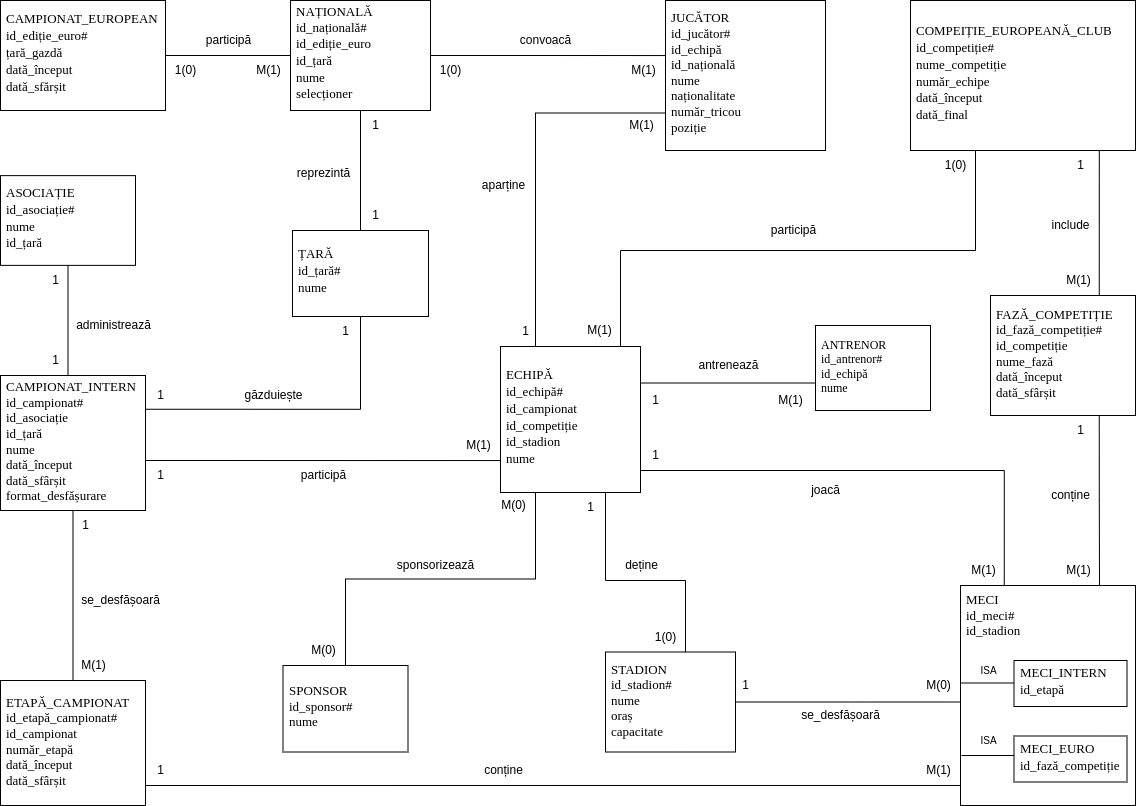
\includegraphics[width=\dimexpr\textwidth+3cm\relax]{diagramaER.png}}\\[0.5cm]
		
		\small Figura 1: Diagrama E/R.
		
	\end{center}
	
	% makebox = creaza o 'cutie' de dimensiunea specificata care cuprinde continutul dat (imaginea)
	% [\textwidth] = latimea cutiei, iar [c] = aliniere centrata
	% relax = comanda de finalizare a expresiei 
	
	\newpage
	
	\section{Diagrama conceptuală}
	
	\vspace{1cm}
	\begin{center}
				
		\makebox[\textwidth][c]{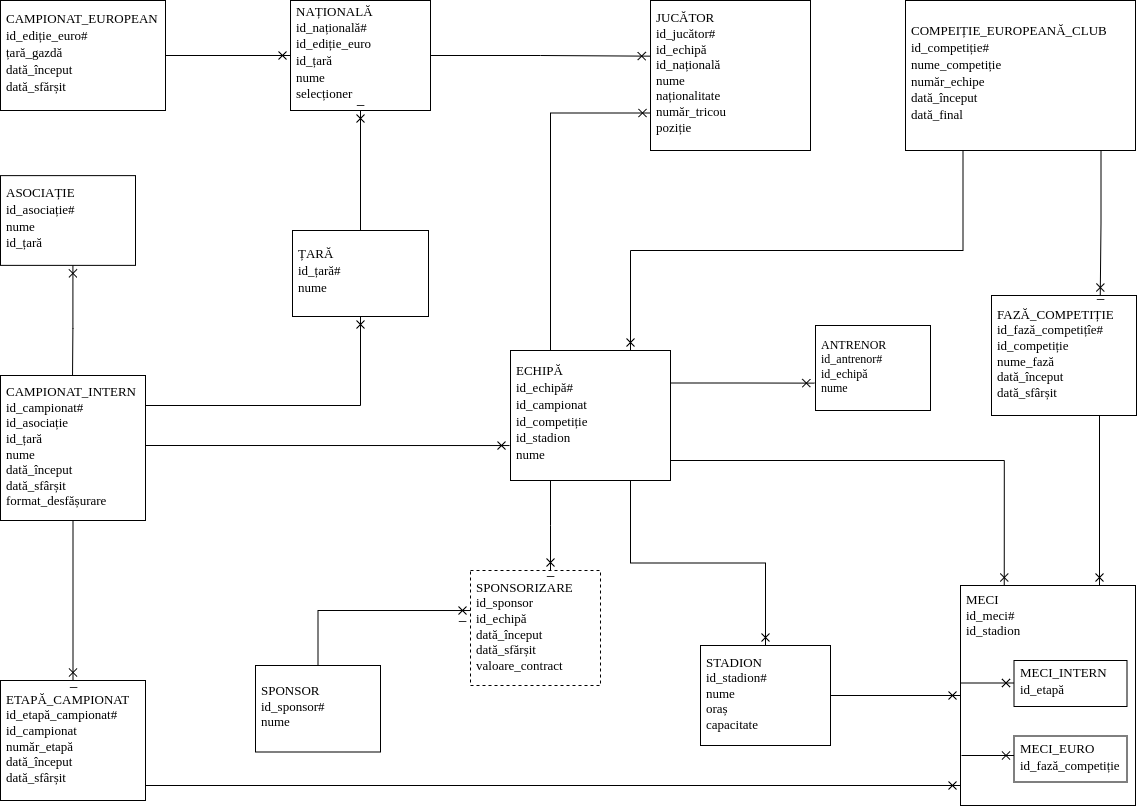
\includegraphics[width=\dimexpr\textwidth+3cm\relax]{diagramaConceptuala.png}}\\[0.5cm]

		\small Figura 2: Diagrama conceptuală.
		
	\end{center}
	
	\newpage

	
	\textbf{Schemele relaționale} corespunzătoare diagramei conceptuale din figura 2 sunt următoarele:
	
	\begin{itemize}[left = 0cm]
		\item[] ȚARĂ(id\_țară\#, nume, cod\_iso);
		
		\item[] ASOCIAȚIE(id\_asociație\#, nume, sediu, id\_țară);
		
		\item[] NAȚIONALĂ(id\_națională\#, id\_ediție\_euro, id\_țară, nume, selecționer);
		
		\item[] CAMPIONAT\_INTERN(id\_campionat\#, id\_asociație, nume, dată\_început, dată\_sfârșit, format\_desfășurare);
		
		\item[] CAMPIONAT\_EUROPEAN(id\_ediție\_euro\#, țară\_gazdă, dată\_început, dată\_sfârșit);
		
		\item[] COMPETIȚIE\_EUROPEANĂ\_CLUB(id\_competiție\#, nume\_competiție, număr\_echipe, dată\_început, dată\_final);
		
		\item[] ETAPĂ\_CAMPIONAT(id\_etapă\_campionat\#, id\_campionat, număr\_etapă, dată\_început, dată\_sfârșit);
		
		\item[] FAZĂ\_COMPETIȚIE(id\_fază\_competiție\#, id\_competiție, nume\_fază, dată\_început, dată\_sfârșit);
		
		\item[] MECI(id\_meci\#, id\_stadion, id\_echipă\_gazdă, id\_echipă\_oaspete, dată);
		
		\item[] MECI\_INTERN(id\_meci\#, id\_etapă);
		
		\item[] MECI\_EURO(id\_meci\#, id\_fază\_competiție, tip\_competiție);
		
		\item[] ECHIPĂ(id\_echipă\#, id\_campionat, id\_competiție, id\_stadion, stadion\_închiriat, nume, oraș, țară);
		
		\item[] STADION(id\_stadion\#, nume, oraș, țară, capacitate);
		
		\item[] JUCĂTOR(id\_jucător\#, id\_echipă, id\_națională, nume, prenume, data\_nașterii, naționalitate, număr\_tricou, poziție, dată\_transfer);
		
		\item[] ANTRENOR(id\_antrenor\#, id\_echipă, nume, prenume);
		
		\item[] SPONSOR(id\_sponsor\#, nume);
		
		\item[] SPONSORIZARE(id\_sponsor, id\_echipă, dată\_început, dată\_sfârșit, valoare\_contract);
		
		
		% nota: sa o intreb pe dna. profesoara daca sunt problematice constrangerile dpdv. al flexibilitatii, raportate la continutul materiei din semestrul curent
		
	\end{itemize}
	
\end{document}